
The project group page is the virtual meeting place described in \secref{sec:projectgroup}.
We decided to implement the room merely as a container for \block{}.
Alternatively the functionality could be an integrated part of the page, but using \block s gives more flexibility to the users allowing them manage the layout of their own project group room. 
A screenshot of a project group room can be seen in \figref{fig:projectgroupnoedit}. 
In this project group room the blocks of the standard layout are seen.
\begin{figure}[h]
	\centering
		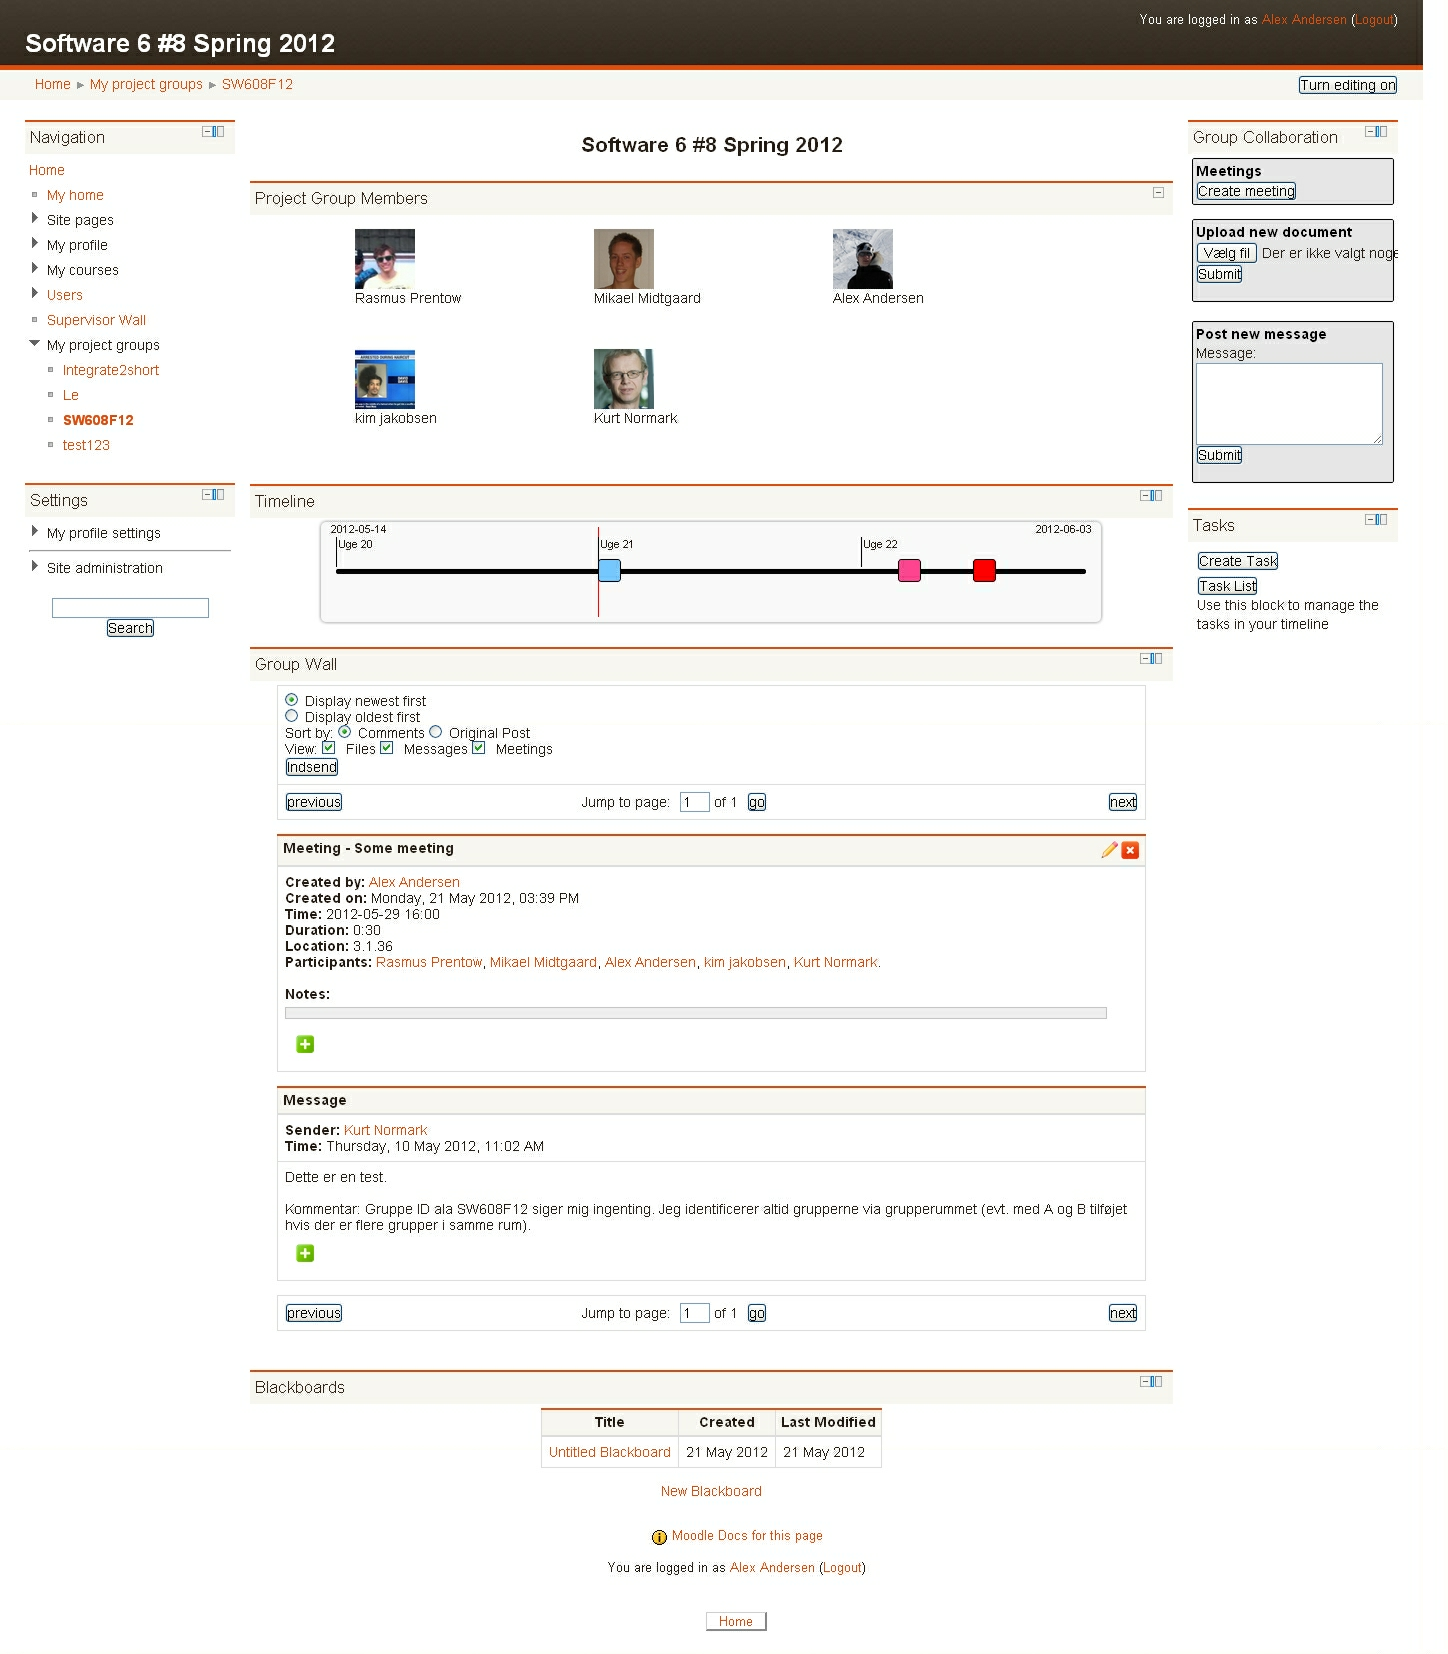
\includegraphics[width=\textwidth]{images/projectgroupnoedit.png}
	\morscaption{The project group room}
	\label{fig:projectgroupnoedit}
\end{figure}

The project group room consist of three columns and three rows. 
The screenshot illustrates the area boundaries by dashed lines. 
%An illustrationThe page in edit mode can be seen in figure \figref{fig:projectgroupwithedit}.
The three rows on the page are from the top; the header, the middle and the footer. 
The header is standard Moodle and is only controlled by us to add a heading. 
The heading shows the name of the project group. 
The middle part is the actual page content and is further divided in three columns. 
The left column is the standard navigation menu in Moodle and is not created by us, though it is extended by us.
%We do not want anything to be added to this column to ensure that the page seem familiar to the user.
The center and right columns both contain blocks.
The center area is much wider than the left and right and can therefore contain bigger \block{}s. 
The various blocks presented on the project groups page are described in \secref{sec:implprojectgroupblocks}. 
If a user wants to edit the layout for the project group room he can press the ``Turn editing on'' button. 
This will add edit and move buttons to each \block{}, allowing the user to remove, add, move, and edit \block{}s. 
A special ``add new block''-block is added in editing mode to allow for adding new \block[]. 
If a user edits the page, the change can be seen by all group members. 

To specify on the figure what a \block{} is we have grayoed out one of the \block{}s.
The grayed out area is the members block and is created by our group. 
The block shows a photo and the name of each member of the group. 



